%%____________________________________________________________________________||
\section{Interpretation in Simplified Dark Matter Models}
\label{sec:DM}

We consider here an interpretation of the results of this search using simplified dark matter models.

\subsection{Signal models}
\label{sec:DM_models}

% TO COVER:
% Simplified models
% Model combinations for Pseudoscalar, scalar
% Generation of signal samples
\begin{figure}[h!]
    \begin{center}
        \subfigure[Heavy Flavour Vector / Axial Vector]{
            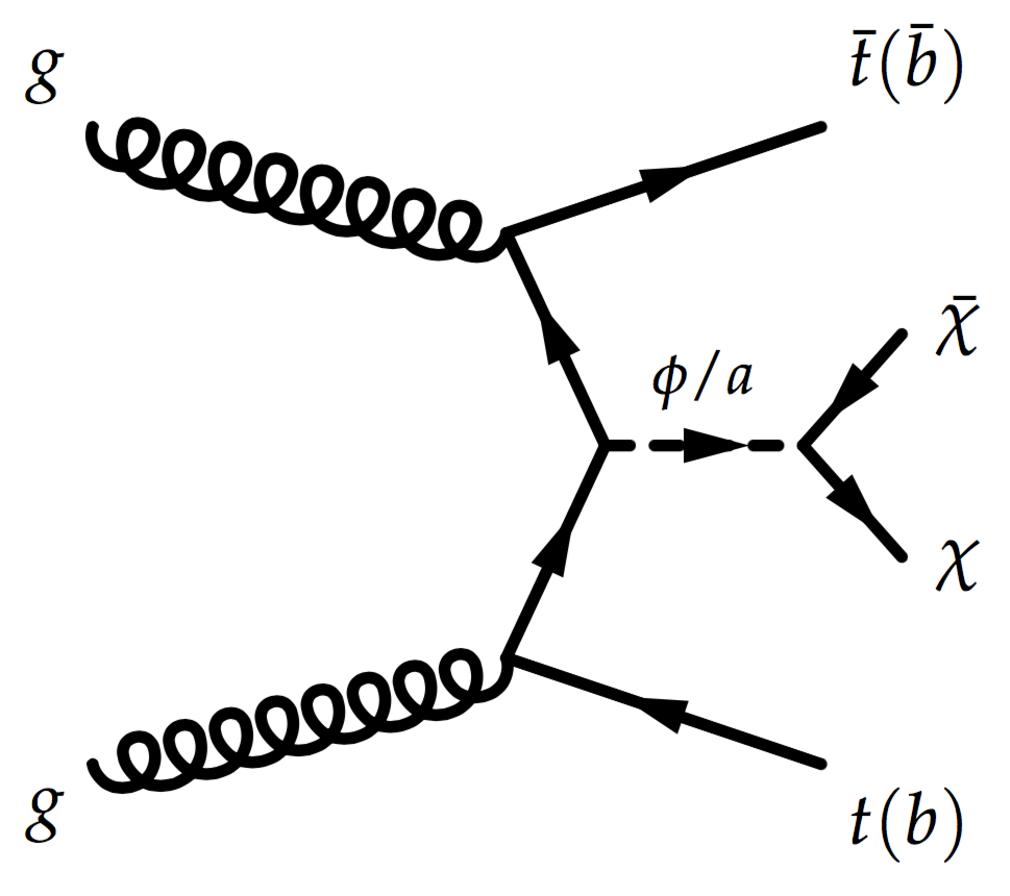
\includegraphics[width=0.3\textwidth]{figures/DMResults/feynman_hf}
            \label{fig:DM-Feynman:HeavyVA}
        }~~
        \subfigure[Light Flavour Vector / Axial Vector]{
            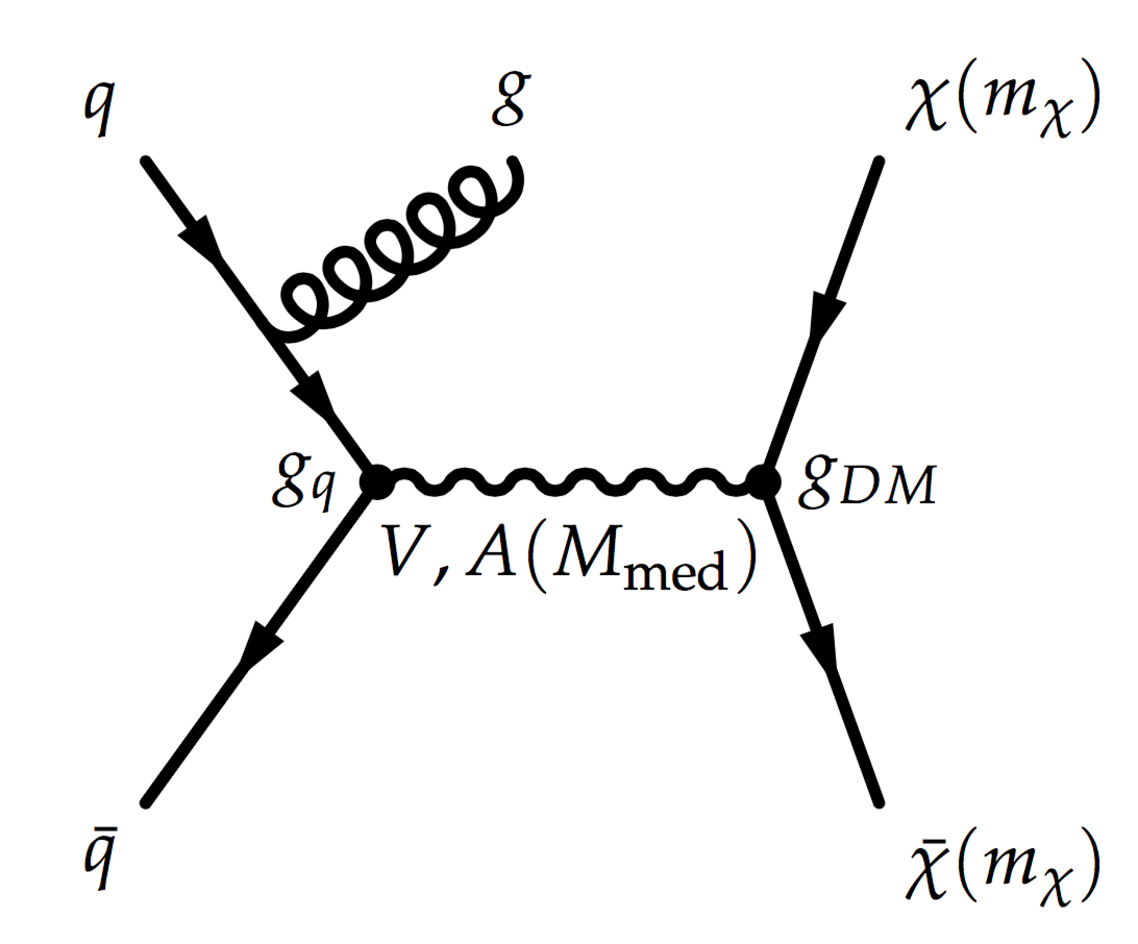
\includegraphics[width=0.3\textwidth]{figures/DMResults/feynman_light_jet}
            \label{fig:DM-Feynman:LightVA}
        }~~
        \subfigure[Light Flavour Scalar / Pseudoscalar]{
		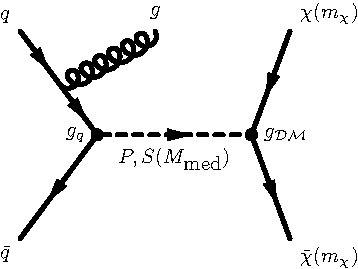
\includegraphics[width=0.3\textwidth]{figures/DMResults/feynman_light_scalar}
            \label{fig:DM-Feynman:LightSP}
        }~~
        \caption{
            Graphical representation of the simplified Dark Matter production models.
        }
        \label{fig:DM-Feynman}
    \end{center}
\end{figure}


\clearpage
\subsection{Signal acceptance times efficiency}
\label{sec:sig-accept-contam-DM}

In Tab. \ref{tab:sig-eff-DM} the signal efficiency is summarised for benchmark
mass points.

\begin{table}[h!]
    \scriptsize
	\caption{Signal efficiency for different DM models.}
    \label{tab:sig-eff-DM}
    \centering
    \begin{tabular}{ lllll }
        \hline \hline
        Model & $(m_{\mathrm{Med}},m_{\mathrm{DM}})$ & Efficiency (total) \\ 
        \hline
        \multirow{2}{*}{ttP}
            & (1700,100) & XXX\% \\
            & (1000,850) & XXX\% \\
        \hline
        \multirow{2}{*}{bbP}
            & (1900,100)  & XXX\% \\
            & (1300,1100) & XXX\% \\
        \hline
        \multirow{2}{*}{qqP}
            & (1700,100) & XXX\% \\
            & (950,600)  & XXX\% \\
        \hline
        \multirow{2}{*}{P - combined}
            & (700,100) & XXX\% \\
            & (400,300) & XXX\% \\
        \multirow{2}{*}{ttP}
            & (1700,100) & XXX\% \\
            & (1000,850) & XXX\% \\
        \hline
        \multirow{2}{*}{bbS}
            & (1900,100)  & XXX\% \\
            & (1300,1100) & XXX\% \\
        \hline
        \multirow{2}{*}{qqS}
            & (1700,100) & XXX\% \\
            & (950,600)  & XXX\% \\
        \hline
        \multirow{2}{*}{S - combined}
            & (700,100) & XXX\% \\
            & (400,300) & XXX\% \\
        \hline
        \multirow{2}{*}{V - combined}
            & (700,100) & XXX\% \\
            & (400,300) & XXX\% \\
        \hline
        \multirow{2}{*}{A - combined}
            & (700,100) & XXX\% \\
            & (400,300) & XXX\% \\
        \hline \hline
    \end{tabular}
\end{table}

% Discuss: Signal contamination of the CRs?

\clearpage
\subsection{Systematic uncertainties on signal efficiency times acceptance}
\label{sec:sig-syst-DM}
% TODO: COPIED DIRECTLY FROM SUSY, Update for DM

The following sources of systematic uncertainty are propagated to the signal
acceptance and shape, according to the recommendations agreed on within the
collaboration. Relative effect on the yields are presented in
Tab.~\ref{tab:sig-systematics-DM} for some benchmark models.

\begin{itemize}
    \item Luminosity: 2.6\%, taken as correlated across all bins.
    \item Trigger: conservatively, the size of the inefficiency is taken as
        systematic variation where not in the plateau (see Sec.~\ref{sec:triggers}).
    \item MC statistics:  uncorrelated bin-by-bin uncertainty, affecting the
        shape of the signal.
    \item Pileup reweighting: 5.0\% uncertainty on the minimum bias cross section
        (see Sec.~\ref{sec:pileup-reweighting}).
    \item b-tag efficiency: uncertainty on the FullSim and FastSim b-tag scale
        factor is propagated and taken as correlated across the bins.
    \item Lepton efficiency: uncertainty on the lepton scale factors is
        propagated and taken as correlated across the bins.
    \item Jet energy scale: uncertainty on the jet energy corrections is
        propagated and taken as correlated across the bins.
    \item Initial State Radiation (ISR): Reweighting of the $N_{\text{isr}}$
        distribution. The systematic is taken as half the corrections.
\end{itemize}

\begin{table}[h!]
        % TODO CHANGE THIS TABLE
    \scriptsize
    \caption{
        Representative range taken from the $16\%$ and $84\%$ percentiles of the
        uncertainty across the analysis bins for each source of signal
        systematic. Two benchmark point are chosen for each model, corresponding
        to ``compressed'' and ``uncompressed'' scenarios, i.e. with small and
        large mass splitting between the mother particle and the LSP. A third
        benchmark is chosen for T2tt for the $W$ corridor and no
        ``uncompressed'' is chosen for T2cc.
    }
    \label{tab:sig-systematics-DM}
    \centering
    \begin{tabular}{ ccccccccc }
        \hline \hline
        Model & ($m_{\mathrm{Susy}},m_{\mathrm{LSP}}$) & Luminosity & ISR & JEC & PU & b-tag & Trigger & MC stat. \\ \hline
        \multirow{2}{*}{T1qqqq}
            & (1700,100) & 2.6\% & 2-4\%  & 2-12\% & 6-12\% & 1-1\% & 1-2\% & 14-19\% \\
            & (1000,850) & 2.6\% & 3-14\% & 5-14\% & 9-14\% & 3-7\% & 2-4\% & 6-22\%  \\
        \hline
        \multirow{2}{*}{T1bbbb}
            & (1900,100)  & 2.6\% & 3-9\%  & 4-6\%  & 7-14\% & 7-12\% & 4-5\% & 11-19\% \\
            & (1300,1100) & 2.6\% & 2-11\% & 3-11\% & 5-9\%  & 2-5\%  & 1-3\% & 11-22\% \\
        \hline
        \multirow{2}{*}{T1tttt}
            & (1700,100) & 2.6\% & 2-6\% & 3-15\%  & 2-9\%  & 2-6\% & 2-4\% & 12-24\% \\
            & (950,600)  & 2.6\% & 5-9\% & 12-26\% & 7-13\% & 2-6\% & 3-7\% & 15-30\% \\
        \hline
        \multirow{2}{*}{T2qq (1-fold)}
            & (700,100) & 2.6\% & 2-7\%  & 3-10\% & 6-9\%  & 0-5\% & 1-4\% & 4-22\% \\
            & (400,300) & 2.6\% & 5-22\% & 5-18\% & 9-15\% & 3-5\% & 3-5\% & 6-20\% \\
        \hline
        \multirow{2}{*}{T2qq (8-fold)}
            & (1250,100) & 2.6\% & 2-7\%  & 5-14\% & 5-10\% & 1-1\% & 1-3\% & 12-24\% \\
            & (700,600)  & 2.6\% & 4-17\% & 4-13\% & 9-14\% & 2-5\% & 2-4\% & 6-22\%  \\
        \hline
        \multirow{2}{*}{T2bb}
            & (1000,100) & 2.6\% & 1-7\%  & 4-11\% & 5-9\%  & 1-4\% & 0-3\% & 14-23\% \\
            & (550,450)  & 2.6\% & 4-15\% & 4-15\% & 8-13\% & 3-7\% & 2-3\% & 9-22\%  \\ 
        \hline
        \multirow{2}{*}{T2tt}
            & (1000,50) & 2.6\% & 3-7\%   & 4-14\% & 6-10\%  & 1-5\%  & 1-4\%  & 14-27\% \\
            & (450,200) & 2.6\% & 4-12\%  & 6-15\% & 10-14\% & 4-9\%  & 3-6\%  & 6-19\%  \\
            & (250,150) & 2.6\% & 13-27\% & 8-22\% & 12-25\% & 6-16\% & 6-17\% & 10-23\% \\
        \hline
        \multirow{1}{*}{T2cc}
            & (500,480) & 2.6\% & 4-18\% & 5-13\% & 5-12\% & 1-4\% & 2-4\% & 6-19\% \\
        \hline \hline
    \end{tabular}
\end{table}

\clearpage
\subsection{Exclusion limits and significance}
\label{sec:DM_results}

In order to extract the signal contribution in the fit, the
distribution of events according to the \mht variable, encoded as
template histograms as described in
Secs.~\ref{sec:htmiss-categorisation}, \ref{sec:mht-intro},
\ref{sec:mht-zinv-intro}, and \ref{sec:likelihood}, is used. Upper
limits on the cross section are computed using the $\text{CL}_{s}$
criterion \cite{CLsTechnique}. Asymptotic formulae
\cite{AsymptoticFormulae} are utilised to approximate the distribution
of the test statistics. All the statistical results are produced using
the \textit{combine} tool, provided within the
HiggsAnalysis-CombinedLimit package \cite{Combine}.

The models are grouped according to the following categorisation:
\begin{itemize}
\item \textbf{Gluino-mediated production of off-shell (decoupled) 3rd
    generation squarks}: gluino pair production followed by 3-body
  decay to $t\bar{t}\chiz$,$b\bar{b}\chiz$.  It includes T1bbbb and
  T1tttt.
\item \textbf{Direct and gluino-mediated production of off-shell
    (decoupled) light-flavour squarks}: gluino/light squark pair
  production followed by 3-body/2-body decay to $q(q)\chiz$. It
  includes T1qqqq and T2qq.
\item \textbf{Direct production of 3rd generation squarks}:
  stop/sbottom pair production, with several possibility for the decay
  (see Tab.~\ref{tab:simplified-models}). It includes T2bb, T2tt and
  T2cc.
\end{itemize}

Table~\ref{tab:dm_aggr_limits} shows the observed and expected limits
determined for the benchmark models using both the nominal and
simplified binning schemes. 

In Figs.~\ref{fig:T1qqqq}-\ref{fig:T2cc} (top) the 95\% C.L. upper
limits on the cross section are shown in the
$(m_{\mathrm{Susy}},m_{\mathrm{LSP}})$ plane for the models considered
in this interpretation. These results correspond to 35.9~\ifb of
integrated luminosity. The exclusion contour is also shown together
with $\pm1\sigma$ (and $\pm2\sigma$ for the expected exclusion)
uncertainty.  The band around the expected exclusion reflects the
experimental uncertainty, while the band around the observed exclusion
correspond to the theoretical uncertainty on the signal cross
section. In Figs.~\ref{fig:T1qqqq}-\ref{fig:T2cc} (left) the signal
acceptance for each mass point in the SMS scan. In
Figs.~\ref{fig:T1qqqq}-\ref{fig:T2cc} (right) each mass point is
assigned a group of 4 jet categories in descending order of
sensitivity. The total number of mass points with the same 4 most
sensitive jet categories is noted. In the gluino production models in
the uncompressed regions the high jet multiplicities drive the
sensitivity (ge6j, eq5j, eq4j), and in the compressed regions the same
high jet multiplicities drive the sensitivity with the asymmetric jet
topologies playing a larger role than in the uncompressed regions. In
the T2qq and T2bb models, the sensitivity in the uncompressed regions
are driven by low/medium jet multiplicities (eq2j, eq3j, eq4j), and in
the compressed regions it's driven by high jet multiplicities (ge6j,
eq5j, eq4j). In stop production models the uncompressed and compressed
regions are driven by high jet multiplicities (ge6j, eq5j, eq4j) with
the asymmetric topology playing a larger role in the compressed
regions.  The weakest jet multiplicity, in terms of limit sensitivity,
is the monojet category and is expected to become sensitive for Dark
matter models. In Figs.~\ref{fig:T1qqqq}-\ref{fig:T2cc} (bottom) the
local observed significance for each mass point in the SMS scan is
shown.

In summary, gluino masses up to $\sim$1800 GeV for the decay into
light-quarks (T1qqqq), $\sim$2050 GeV for the decay into b-quarks
(T1bbbb) and $\sim$1850 GeV for the decay into t-quarks
(T1tttt). Squark production is excluded up to squark masses $\sim$1400
GeV for the 8-fold models, and up to $\sim$800 GeV for the 1-fold
(degenerate) models (T2qq). Sbottom production is excluded to sbottom
masses $\sim$1100 GeV (T2bb).  Stop production is excluded up to stop
masses $\sim$1050 GeV in the 2-body decay to top quarks (T2tt), and up
to $\sim$550 GeV in the compressed region of decays into charm quarks
(T2cc).  For the models considered, the exclusion exceeds the one of
the 13 TeV ICHEP data.

\begin{table*}[!t]
  \topcaption{Expected ($\mu_{\text{exp}}$) and observed 
    ($\mu_{\text{obs}}$) upper limits on the production cross section, 
    expressed in terms of the signal strength parameter, obtained using
    both the nominal and simplified binning schema. 
  }
  \label{tab:dm_aggr_limits}
  \centering
  \begin{tabular}{ llccccc }
    \hline
    \multicolumn{2}{c}{Benchmark models}    & \multicolumn{2}{c}{Nominal}
                                            & 
                                            & \multicolumn{2}{c}{Simplified}             \\ [0.3ex]
    \cline{3-4}
    \cline{6-7}
   \multicolumn{2}{c}{$(m_{\text{Med}}, m_{\mathrm{DM}})$ [\GeVns{}]} 
                                            & $\mu_{\text{exp}}$
                                            & $\mu_{\text{obs}}$
                                            & 
                                            & $\mu_{\text{exp}}$
                                            & $\mu_{\text{obs}}$                         \\ [0.3ex]
    \hline
    \multirow{1}{*}{ttP} & (XXX, XXX)  & XXX & XXX &  & XXX & XXX \\
    \multirow{1}{*}{bbP} & (XXX, XXX)  & XXX & XXX &  & XXX & XXX \\
    \multirow{1}{*}{qqP} & (XXX, XXX)  & XXX & XXX &  & XXX & XXX \\
    \multirow{1}{*}{P}   & (XXX, XXX)  & XXX & XXX &  & XXX & XXX \\
    \multirow{1}{*}{ttS} & (XXX, XXX)  & XXX & XXX &  & XXX & XXX \\
    \multirow{1}{*}{bbS} & (XXX, XXX)  & XXX & XXX &  & XXX & XXX \\
    \multirow{1}{*}{qqS} & (XXX, XXX)  & XXX & XXX &  & XXX & XXX \\
    \multirow{1}{*}{S}   & (XXX, XXX)  & XXX & XXX &  & XXX & XXX \\
    \multirow{1}{*}{qqV} & (XXX, XXX)  & XXX & XXX &  & XXX & XXX \\
    \multirow{1}{*}{qqA} & (XXX, XXX)  & XXX & XXX &  & XXX & XXX \\
    \hline
  \end{tabular}
\end{table*}

%Summary exclusion plots according to this categorisation are presented in
%Fig.~\ref{fig:summary-excl-plots}.

% TODO: Uncomment and add plots for different models below:
%\newpage
%\begin{figure}[h!]
%    \begin{center}
%        \subfigure[Pseudoscalar: Upper limit on the cross section in the mass plane]{
%            \includegraphics[width=0.6\textwidth]{figures/DMResults/DMP_XSEC}
%            \label{fig:DMP_excl}
%        } \\
%        \subfigure[Pseudoscalar: $\epsilon_{sig}$]{
%            \includegraphics[width=0.45\textwidth]{figures/DMResults/DMP_effs}
%            \label{fig:DMP_eff}
%        } ~~
%        \subfigure[Pseudoscalar: Most sensitive categories]{
%            \includegraphics[width=0.45\textwidth]{figures/DMResults/DMP_bitMap}
%            \label{fig:DMP_bitMap}
%        } \\
%        \subfigure[Pseudoscalar: Significance scan]{
%            \includegraphics[width=0.45\linewidth]{figures/DMResults/DMP_signif}
%            \label{fig:DMP_signif}
%        } ~~
%        \caption{Top: the 95\% C.L. observed upper limit on the cross section
%            (histogram), with the expected (solid black line) observed
%            (solid red line) exclusion contours. Left: signal acceptance
%            including all jet categories. Right: graph showing the four
%            most sensitive jet categories for each mass point. Bottom:
%            local observed significance scan.
%        }
%        \label{fig:DMP}
%    \end{center}
%\end{figure}
